\documentclass[11pt]{article}
\usepackage[margin=1in]{geometry}
\usepackage{graphicx}
\usepackage{booktabs}
\usepackage{longtable}
\usepackage{array}
\usepackage{hyperref}
\usepackage{enumitem}
\usepackage{titlesec}
\usepackage{xcolor}

\titleformat{\section}{\large\bfseries}{\thesection}{0.6em}{}
\titleformat{\subsection}{\normalsize\bfseries}{\thesubsection}{0.6em}{}
\setlist[itemize]{leftmargin=1.4em}
\hypersetup{colorlinks=true,urlcolor=blue,linkcolor=black}

\title{Landscape Assessment: Commercialization Viability Tooling for\newline Venture Capital and University OTM Workflows}
\author{Prepared for Avi}
\date{31 March 2026}

\begin{document}
\maketitle

\section{Purpose and Scope}
This report maps the current tool landscape used by:
\begin{itemize}
    \item Venture Capital firms for startup screening and diligence, and
    \item University Offices of Technology Management (OTM/TTO) for invention intake, IP operations, and commercialization decisions.
\end{itemize}

The report identifies where current platforms stop, where process gaps remain, and where a dedicated commercialization viability platform can intervene with a defensible product position.

\section{Executive Findings}
\begin{itemize}
    \item The market is segmented. VC teams and OTM teams assemble multiple tools across CRM, market intelligence, patent analytics, publication intelligence, and compliance systems.
    \item No reviewed production platform provides one native workflow that combines: patent intelligence, scientific evidence quality, market sizing, competitor mapping, and commercialization viability scoring.
    \item OTM commercialization triage is still human-led at critical decision points, including assignment, patent filing decisions, licensing path decisions, and conflict review.
    \item The strongest intervention point is a governance-grade decision engine that integrates into existing OTM systems and outputs investor-ready diligence artifacts.
\end{itemize}

\section{Detailed Scoping: Venture Capital Tooling}

\subsection{Representative Platforms}
\begin{longtable}{p{0.14\textwidth} p{0.11\textwidth} p{0.23\textwidth} p{0.21\textwidth} p{0.25\textwidth}}
\toprule
\textbf{Logo} & \textbf{Platform} & \textbf{Primary Use in VC Workflow} & \textbf{Strengths} & \textbf{Observed Gap Relative to Target Product} \\
\midrule
\endhead

\includegraphics[width=0.11\textwidth]{report_assets/cbinsights.png} & CB Insights & Private company discovery, market and competitor intelligence, predictive indicators & Broad company and market signal coverage; widely used by investment and strategy teams & Limited evidence-quality scoring at publication level and no integrated claim-level IP + scientific + commercialization score in one workflow \\


\includegraphics[width=0.11\textwidth]{report_assets/dealroom.png} & Dealroom & Startup and ecosystem discovery, tracking, exports and workflow feeds & Useful for ecosystem mapping and company tracking & Not designed as a science quality and patent-depth commercialization scoring engine \\


\includegraphics[width=0.11\textwidth]{report_assets/tracxn.png} & Tracxn & Startup and investor dataset platform with workflow support & Strong taxonomy and discovery support for sectors and firms & Data-centric platform, not an integrated university deep-tech viability scoring platform \\


\includegraphics[width=0.11\textwidth]{report_assets/patsnap.png} & PatSnap & Patent intelligence and technology landscape analysis & Strong IP analytics and portfolio-level patent visibility & Not a full system for market sizing, scientific evidence quality grading, and end-to-end commercialization scoring \\

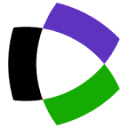
\includegraphics[width=0.11\textwidth]{report_assets/clarivate.png} & Clarivate Derwent & Patent portfolio analytics, prosecution and citation context & Strong IP and legal intelligence depth & Oriented to IP analytics, not integrated with investor-market and science-quality scoring in one decision stack \\


\includegraphics[width=0.11\textwidth]{report_assets/lens.png} & Lens & Scholarly and patent discovery and link analysis & Good patent-literature linkage and broad discovery coverage & Requires analyst interpretation; no native commercialization decision score workflow \\


\includegraphics[width=0.11\textwidth]{report_assets/cas.png} & CAS SciFinder & Scientific and patent intelligence, especially in chemistry and life sciences & Deep domain retrieval quality for scientific intelligence & Research intelligence layer only; not an OTM or VC commercialization execution system \\
\bottomrule
\end{longtable}

\subsection{VC Workflow Conclusion}
VC tooling is mature in components but not in integrated decision synthesis for university-origin deep tech. Teams still stitch outputs manually across data products, IP tools, and technical diligence providers.

\section{Detailed Scoping: OTM/TTO Tooling Across Universities}

\subsection{Representative Platforms and Infrastructure}
\begin{longtable}{p{0.14\textwidth} p{0.11\textwidth} p{0.23\textwidth} p{0.21\textwidth} p{0.25\textwidth}}
\toprule
\textbf{Logo} & \textbf{Platform} & \textbf{Primary Use in OTM Workflow} & \textbf{Strengths} & \textbf{Observed Gap Relative to Target Product} \\
\midrule
\endhead

\includegraphics[width=0.11\textwidth]{report_assets/inteum.png} & Inteum Minuet & Disclosure intake, docketing, agreements, portfolio and compliance workflow support & Strong system-of-record capabilities for TTO operations and process control & AI features are assistive; does not replace commercialization triage with integrated market plus science plus IP scoring \\


\includegraphics[width=0.11\textwidth]{report_assets/wellspring.png} & Wellspring & Innovation and IP workflow support for transfer offices and institutions & Established presence in innovation management category & Publicly visible detail indicates platform breadth, but no evidence of full automated commercialization viability scoring stack \\


\includegraphics[width=0.11\textwidth]{report_assets/autm.png} & AUTM STATT / TransACT & Benchmarking data and transaction support references for member institutions & Valuable benchmarking and precedent support for negotiations & Not an operational workflow system and not a real-time triage decision engine \\


\includegraphics[width=0.11\textwidth]{report_assets/inpart.png} & IN-PART & University to industry opportunity discovery and partner matching & Improves external partner reach and campaign visibility & Upstream quality filter and internal commercialization scoring still required before outreach \\


\includegraphics[width=0.11\textwidth]{report_assets/firstignite.png} & FirstIgnite & AI-assisted partner matching for licensing and sponsored research leads & Useful for external match discovery & Not a replacement for IP compliance systems, prosecution decisions, or committee-level commercialization scoring \\
\bottomrule
\end{longtable}

\subsection{Regulatory and Process Baseline}
US universities handling federally funded inventions must comply with Bayh-Dole reporting through iEdison and associated regulatory timelines. These obligations reinforce structured operations but do not provide commercialization scoring or investor-grade viability analysis.

\section{Evidence of Manual Commercialization Triage}
Observed workflow evidence from university process documentation indicates manual decision points remain central:
\begin{enumerate}
    \item Case assignment to licensing managers.
    \item Human judgment on patent filing and continuation decisions.
    \item Human selection of licensing strategy and negotiation posture.
    \item Conflict-of-interest and governance review before deal execution.
    \item Manual prioritization due to low disclosure-to-license conversion rates.
\end{enumerate}

This is the critical operational gap where automation can improve consistency and speed without removing accountable human oversight.

\section{Gap Taxonomy and Intervention Opportunities}
\subsection{Gap Taxonomy}
\begin{itemize}
    \item \textbf{Workflow fragmentation gap}: VC and OTM systems are not connected by a shared decision layer.
    \item \textbf{Readiness framework gap}: TRL or status views are common, but composite commercialization readiness scoring is not standardized.
    \item \textbf{Evidence normalization gap}: disclosures, patents, literature, and market data are not converted into one traceable evidence model.
    \item \textbf{Benchmarking gap}: sparse comparative baselines for university-stage assets by domain and stage.
    \item \textbf{Governance gap}: limited versioned decision logs, override reasoning, and auditable scoring histories.
    \item \textbf{Actionability gap}: few systems prescribe next de-risking actions with expected impact and effort.
\end{itemize}

\subsection{Intervention Model}
\textbf{Positioning:} Build a commercialization viability decision engine that sits between OTM systems of record and downstream investor or partner diligence workflows.

\textbf{Core outputs:}
\begin{itemize}
    \item Explainable composite viability score with confidence level.
    \item Citation-backed evidence map covering IP, science quality, market and competition.
    \item Prioritized de-risking action plan with expected score lift.
    \item Committee-grade decision packet and audit trail.
\end{itemize}

\section{Phased Build Plan}
\subsection{MVP (0 to 4 months)}
\begin{itemize}
    \item Read-only connectors to one OTM source plus CSV fallback.
    \item Scoring ontology across technical maturity, market validation, IP defensibility, regulatory path, scale feasibility, and team readiness.
    \item Evidence extraction with source traceability and confidence flags.
    \item One-page commercialization brief and structured appendix.
\end{itemize}

\subsection{Phase 2 (5 to 10 months)}
\begin{itemize}
    \item Bidirectional workflow integration with selected OTM stack.
    \item Benchmarking by domain and development stage.
    \item Portfolio triage cockpit and decision governance module.
\end{itemize}

\subsection{Phase 3 (11 to 18 months)}
\begin{itemize}
    \item Cross-institution benchmark intelligence with privacy controls.
    \item Predictive conversion modeling for license and startup progression.
    \item Counterparty-ready diligence outputs for VC and strategic partners.
\end{itemize}

\section{Risk Register and Mitigation}
\begin{longtable}{p{0.29\textwidth} p{0.31\textwidth} p{0.34\textwidth}}
\toprule
\textbf{Risk} & \textbf{Operational Impact} & \textbf{Mitigation} \\
\midrule
\endhead
Model credibility risk & Low trust in score outputs & Explainable scoring components, citation traceability, domain calibration reviews \\
Data quality heterogeneity & Inconsistent assessments & Confidence levels, minimum data thresholds, ingestion quality checks \\
Institutional adoption friction & Slow rollout and low usage & Shadow mode pilot, human final signoff, configurable rubric weights \\
Security and confidentiality exposure & Legal and reputational impact & Tenant isolation, encryption, RBAC, contractual data boundaries, audit logging \\
Integration dependency changes & Workflow breaks and maintenance cost & Adapter architecture, fallback import paths, connector monitoring \\
\bottomrule
\end{longtable}

\section{Recommended Pilot Design}
\begin{itemize}
    \item \textbf{Pilot site:} one research university, OTM plus one translational funding committee.
    \item \textbf{Cohorts:} 80 to 120 treatment disclosures with matched baseline comparison.
    \item \textbf{Duration:} minimum two quarters, target nine months.
\end{itemize}

\textbf{Primary KPIs}
\begin{itemize}
    \item Median cycle time from disclosure to triage decision.
    \item Inter-reviewer consistency on readiness dimensions.
    \item Evidence completeness at decision point.
    \item Share of cases with explicit de-risking action plans.
    \item Early conversion lift to license or startup diligence gate.
\end{itemize}

\section{Conclusion}
Your working thesis is supported by market evidence. Current tools are capable in isolated functions but do not deliver integrated commercialization viability assessment for university-origin technologies. A product that combines explainable scoring, evidence traceability, governance controls, and workflow integration can address an operationally real gap for both OTM offices and deep-tech investors.

\section*{References}
\small
\begin{itemize}
    \item CB Insights platform and pricing pages: \url{https://www.cbinsights.com/what-we-offer/platform/}, \url{https://www.cbinsights.com/what-we-offer/pricing/}
    \item Dealroom platform and pricing: \url{https://dealroom.co/platform}, \url{https://dealroom.co/pricing/}
    \item Tracxn pricing: \url{https://tracxn.com/pricing}
    \item PatSnap investor solutions: \url{https://www.patsnap.com/solutions/business-solutions/investor-solutions/}
    \item Clarivate Derwent analytics: \url{https://clarivate.com/intellectual-property/derwent/patent-analytics/}
    \item Lens platform: \url{https://www.lens.org/}
    \item CAS SciFinder: \url{https://www.cas.org/solutions/cas-scifinder-discovery-platform}
    \item Inteum and Minuet pages: \url{https://www.inteum.com/}, \url{https://www.inteum.com/minuet/}
    \item Wellspring pages: \url{https://www.wellspring.com/}, \url{https://www.wellspring.com/customers}
    \item AUTM databases: \url{https://autm.net/surveys-and-tools/databases}
    \item NIST iEdison: \url{https://www.nist.gov/iedison}
    \item eCFR 37 CFR 401.14: \url{https://www.ecfr.gov/current/title-37/chapter-IV/part-401/section-401.14}
    \item IN-PART for universities: \url{https://in-part.com/for-universities/}
    \item Stanford OTL process and TechFinder: \url{https://otl.stanford.edu/researchers/otls-process}, \url{https://techfinder.stanford.edu}
    \item FirstIgnite universities: \url{https://www.firstignite.com/universities/}
\end{itemize}

\end{document}
